\documentclass[12pt]{article}
\usepackage[T1]{fontenc}
\usepackage[utf8]{inputenc}
\usepackage[margin=20mm]{geometry}
\usepackage{amsmath,color,amsthm,enumerate,amsfonts,mathtools}
\usepackage{graphicx}
\usepackage{enumerate}
\usepackage{amsfonts}
\usepackage{paralist}
\usepackage{stmaryrd}

\newcommand{\done}{\textcolor{blue}{done}}
\newcommand{\tba}{\textcolor{red}{to be addresssed}}

\setlength{\parindent}{0ex}
\setlength{\parskip}{1ex}

\begin{document}

\subsection*{Graph Product Structure for Non-Minor-Closed Classes\\
Vida Dujmovi\'c, Pat Morin, David R. Wood\\
Journal of Combinatorial Theory Series B (JCTB9758)\\
Response to Referee Reports}
		
\subsection*{Referee \#1}

This paper proves that if a class of graphs F admits a product structure
theorem, then the class of all graphs which have a 1-subdivision in F admits
a product structure theorem as well. The main theorem, Theorem 3, while
equivalent to the above statement using standard techniques, is stated in
a different way which is considerably more useful for applications and for
obtaining good bounds. As applications of Theorem 3, the paper shows that
the following classes admit a product structure theorem:

\begin{itemize}
\item graphs drawn on a fixed surface with each edge in $\leq k$ crossings,
\item map graphs of degree $\leq k$ graphs embedded in a fixed surface,
\item string graphs with each curve in $\leq k$ intersections,
\item $k$-nearest neighbour graphs in the plane, and
\item powers of classes of graphs of degree $\leq k$ which admit a product structure theorem.
\end{itemize}

All but the last bullet point are shown to follow from the first.
The main results in the paper are correct, strong, and of high interest,
and the paper should definitely be accepted to JCTB after some
(fairly significant) revisions. In particular, the proof of Theorem 3 is
difficult to read due to the notation, and the paper could be substantially
streamlined without losing the above results. Detailed suggestions follow.

Major comments:

1. Lemma 3: This lemma is really about ``normalised'' tree decompositions, and says that for each $x \in V(T)$, the set $V(T_x)$ has at most $t$ neighbours in $H$. Call this property (T3) and remove (Y1)  through (Y5), which should now be obvious.

\tba

2. Proof of Theorem 9: There is too much notation throughout. As
one example, it is hard to remember which of $T_x$, $Y_x$, $V_x$, $F_x$, $N_x$,
$S_x$, $X_v$, $B_x$, $C_x$ is which. If $\phi(S)$ is written for the subset of $V(G)$
corresponding to a set $S \subseteq V(H)$ and appropriate shorthand and
standard notation for neighbourhoods are used, then $Y_x$, $V_x$, $F_x$, and
$N_x$ can be replaced by $\phi(x)$, $\phi(T_x)$, $N(\phi(T_x))$, and $V(G) \setminus N[\phi(T_x)]$.
The set $X_v$ is only used in the statement of Claim~1, so it does not
need a name; say what these vertices are explicitly. It may be more
indicative to write $\phi'(x)$ for $S_x$ and $B'_x$ for $C_x$.

\tba

3. Theorem 10: Unfortunately I have to suggest removing it. I don’t see
the motivation for making $H$ planar or for improving the constants.
Are the improved constants at all close to tight? Is there another
reason for including it?

\tba

4. Sections 4 and 5: I think as they are currently organized they distract from the purpose of the paper, as stated in the introduction, to ``prove product structure theorems for several non-minor-closed classes of interest.'' Which of Corollaries 1--4 and Theorems 12--17 are most important? I would remove any mention of the applications from the examples section, put that section first, and state in that section a single main theorem with all of the best bounds on the product structure. The applications section is mostly a survey and I think should be focused on the most exciting new corollaries. Theorems 18 and 19 should be in the applications section.

\tba

1. abstract: ``This leads to analogous results for map graphs, string graphs, graph powers, and nearest neighbour graphs.'' $\longrightarrow$ 
Add ``certain types of'' or be more specific. Same comment for immediately after Theorem 4.

\done

2. page 1: ``A tree-decomposition $T$ consists of a tree $T$ and a collection
$T$ '' $\longrightarrow$ Delete the first $T$ and define a $T$-decomposition.

\done

Other comments:

1. abstract: “This leads to analogous results for map graphs, string graphs, graph powers, and nearest neighbour graphs.” $\longrightarrow$ Add “certain types of” or be more specific. Same comment for immediately after Theorem 4.

2. page 1: “A tree-decomposition T consists of a tree T and a collection
T ” $\longrightarrow$ Delete the first T and define a T-decomposition.
>>>>>>> f2dea7a16f3c0af4014722c98524e5a9481eb01b

3. pages 2 – 4: The paragraph following Theorem 2 and Section 1.3
(except for the fact that the apex assumption is necessary) is repetition
of things discussed earlier on in the introduction.

\tba

4. page 6, line 14: ``Thus, it suffices to construct width-$t$ tree decomposition that satisfies (T2).'' $\longrightarrow$ should be (T1)

\done

5. page 6, line 16: ``Select any node $x \in V (T_0)$'' $\longrightarrow$ ``Select any nonempty node $x \in V (T_0)$''

\tba

6. page 6, last paragraph of Lemma 2: This isn’t quite right since you
have to be careful with $x_0$.

\tba

7. page 8, item (i): ``$S$ has small layered width with respect to the layering
L'' $\longrightarrow$ ``$S$ has small layered width with respect to the layering $L$ of
$G$''. Perhaps mention something about how it is easy to find the new layering.

\tba

8. general comment: Claims 1, 2, and 4 are especially belaboured by
notation as they are quite straightforward.

\tba

9. page 8, line 10: ``We say that a vertex $w \in Y_x$ contributes a vertex
$v \in S_x$ if $v$ participates in $x$.'' This needs to be fixed.

\tba

10. page 10, Claim 5: Indices could mostly be removed by continuing
to talk about $T$-ancestors instead. Move the definition of $H+$ and its
directed version up, along with the explanation of what will be proven,
so that it isn’t necessary to define the $s_i$.

\tba

11. page 10, Claim 5: The name $Pww'$ is strange since in case 2. there is
no $w'$ defined.

\done

12. page 11, first paragraph of Section 3: ``This section applies our main results for shortcut systems to prove graph product structure theorem...'' $\longrightarrow$ ``to prove a graph product structure theorem...''

\done

\subsection*{Referee \#2}

The Graph Product Structure Theorem of Dujmović, Joret,
Micek, Morin, Ueckerdt, and Wood (FOCS '19) asserts that every planar
graph is a subgraph of the strong product of a graph of treewidth at
most 8 and a path.  This has been the key tool in resolving several
longstanding open problems on planar graphs (and graphs in
minor-closed classes), including problems on queue layouts,
non-repetitive colouring, $p$-centered colouring, and universal graphs.
This paper extends the Graph Product Structure Theorem beyond
minor-closed classes.  The authors prove product structure theorems
for k-planar graphs, map graphs, string graphs, graph powers, and
nearest neighbour graphs.   The authors also present several
applications of their results.  These are essentially the same
applications as for the original Graph Product Structure Theorem; the
point being that the applications typically follow quite easily once a
product structure theorem is established.

This paper is a significant step in answering the (ambitious) question
of which graph classes admit product structure theorems. It is
extremely well-written (with very few typos) and was a pleasure to
read.  It is certainly well within the scope of JCTB and I strongly
recommend it for acceptance.

Below are some typos and suggestions for the authors.

Page 3.  The sentence 'For each $vw \in E(G')$ there is a path $P$ in $G$
between $v$ and we of length at most $k+1$'' is correct but should be made
more precise.  For example, there could be a short path between $v$ and
$w$ which does not involve any new dummy vertices.  You mean to say that
the 'subdivided path' between $v$ and $w$ has length at most $k+1$.

\done

Page 3.  You should add the assumption that no three edges cross at
the same point (which you can assume by perturbing the embedding).
Otherwise, you will not get a $(k+1, 2)$-shortcut system.

\done

Page 6. Regarding (T1), technically a subtree of a rooted tree can be
rooted at any vertex, so it is a bit imprecise to say that $T[x]$ is
rooted at $x$.  I suggest adding that a subtree of a tree rooted at $r$,
is always considered to be rooted at the vertex closest to $r$.

\done

Page 6. Replace 'that satisfies (T2)' by 'that satisfies (T1)'.

\done

Page 6. Replace 'parent in $T'$ by 'parent in $T_0$'.

\done

Page 6. The term 'hierarchical decomposition' is not defined.

\textcolor{blue}{We have put `hierarchical' in quotes to indicate it is not a defined word.}

Page 7. Although it is clear for me, 'separation' has not been
defined.  Perhaps a blanket note saying all undefined terms are in
Diestel's textbook should be added.

\done

=======
Page 7.  In the very last sentence, I think $B_{x_i}$ should be $B_{z_i}$
(twice).  Moreover, the way the proof is written, it seems to suggest
that we only get that $a \in B_{z_i}$ for each $i \in \{1, \dots, r\}$.
The conclusion that $a \in B_{z_i}$ for each $i \in \{0, \dots, r\}$ is
true though.  In a normalized tree decomposition, if $xy$ is an edge and
$x$ is a $T$-ancestor of $y$, then $x$ must be in $B_y$ (since the subtrees $T_x$
and $T_y$ intersect).

\tba

Page 8.  Can you add a brief explanation why $\mathcal{S}$ is a
partition of $V(G)$?  It is clear that the sets in $\mathcal{S}$ are
disjoint, but why do they cover $V(G)$?

\tba

Page 11. Replace 'belong to $F_\delta'$ by 'belongs to $F_\delta$'.

\done

Page 11. In footnote 11, what the authors call a 'closed curve' I
would call just a 'curve'.  To me, a closed curve satisfies the
additional condition that $f(0)=f(1)$.

\done

Page 13. Could it be that the subgraph induced by the vertices of a
kite is a $K_4$ with some parallel edges?  This seems relevant later in
the proof.

\tba

Page 13. Perhaps I am misunderstanding something, but I do not see why
'none of the edges $vx$, $xw$, $wy$, or $yv$ are crossed by any other edges of
$G$.'  For example, see the attached PDF for a picture where $vw$, $xw$, $wy$,
and $yv$ are all crossed by other edges of $G$.

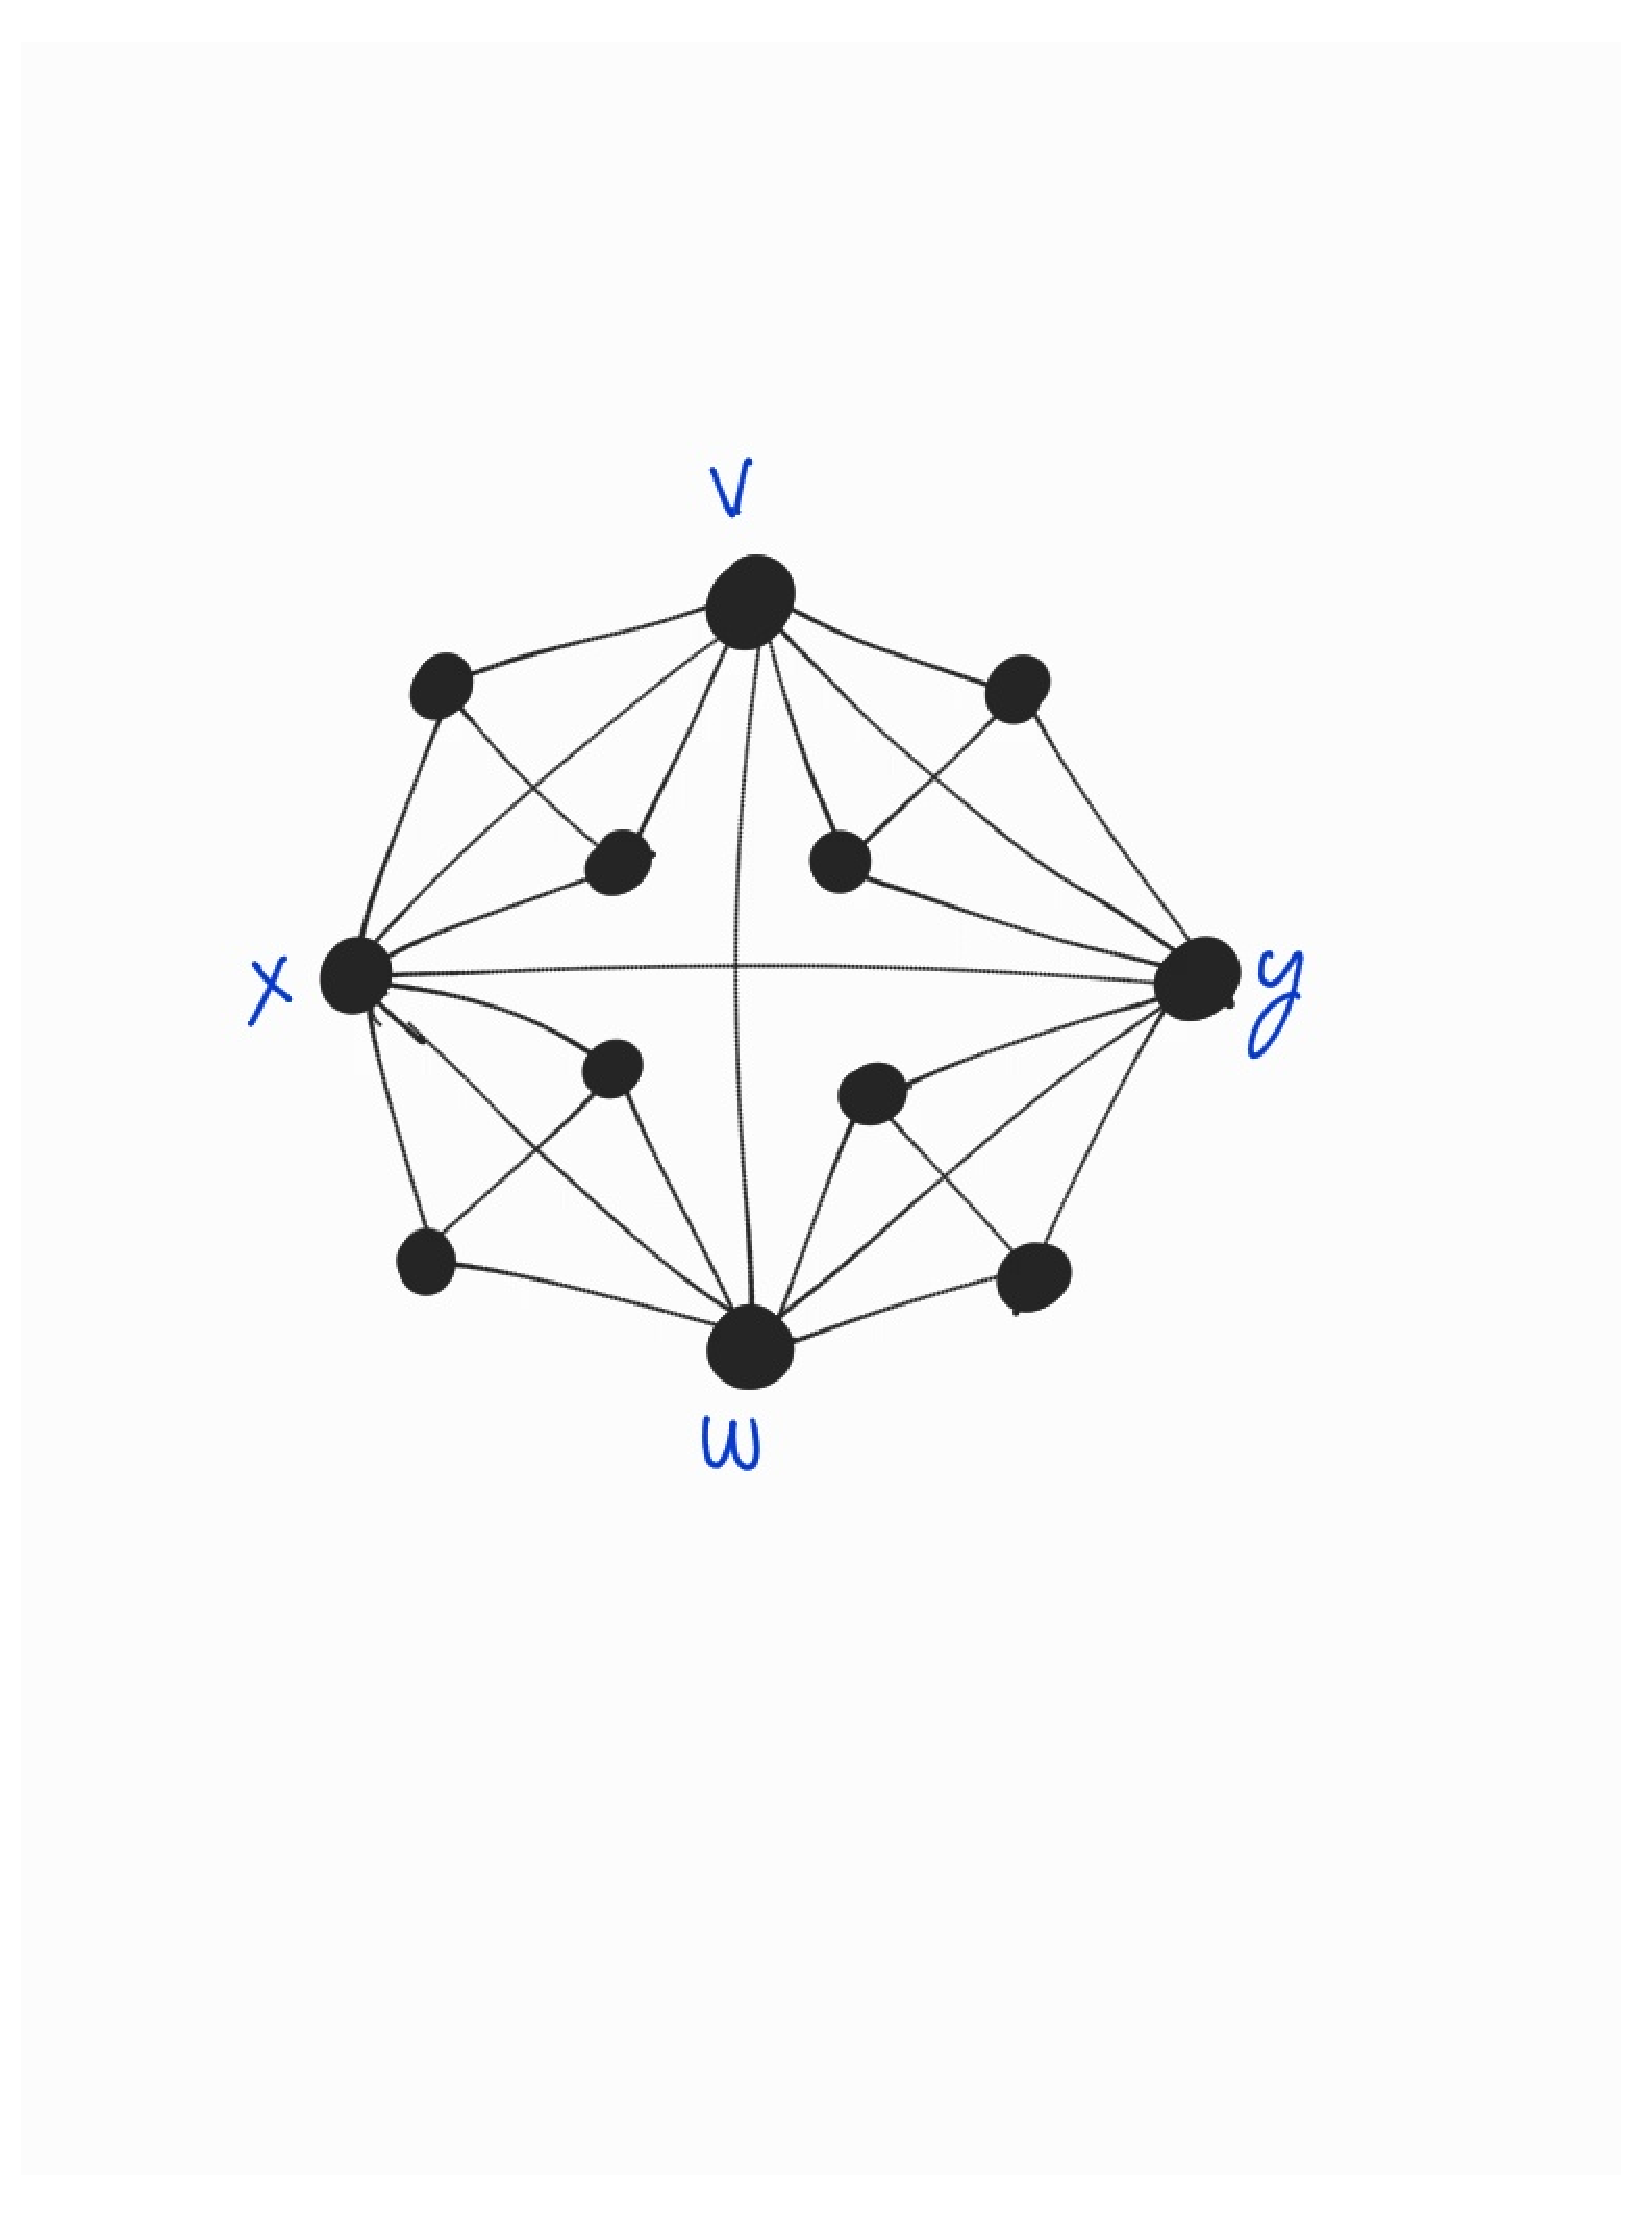
\includegraphics[width=60mm]{kite}

Page 13. The attached PDF also shows that the definition of 'kite
face' may not be well-defined.  For example, I do not see why there
cannot be some edges of $G$ 'inside' a kite face.  Even if this is not
the case, I think it is more precise to say that a kite face has 'two
and a half edges' and two vertices of $G$ on its boundary' rather than
'three edges and two vertices of $G$ on its boundary'.

\tba

Page 13.  Regarding the proof of Lemma 4, I think it is better to
include all the details from reference [14].  As far as I know, JCTB
does not have a page limit, so I do not see an issue with just
reproducing the entire proof and telling the reader that they can skip
all the details if they wish.  This is just my personal opinion
though, so the authors can ignore this request if they choose.

\tba

Page 15. Regarding the proof of Theorem 11, if it really is the same
proof as the proof of Theorem 2, why not just prove Theorem 11 (from
which Theorem 2 follows as a special case)?

\textcolor{blue}{We have written the entire paper starting with simpler cases before moving onto the more general. This approach may use a few more words, but we think the paper becomes more accessible for more readers this way.}

Page 16.  At the end of Page 16, I do not see why 'every pair of edges
cross at most once.'  Without further assumptions, it seems as if two
paths in the path system could intersect several times.  Therefore, by
drawing 'each edge vw of G alongside $P_vw$ in $G_0$', there may be two
edges which cross several times.  It seems this can be fixed by
choosing the path system carefully by 'uncrossing' paths which
intersect at more than two internal vertices.

\tba

Page 18. In point 1 in the proof of Lemma 9, I think '$\phi(w)$' should
be '$\alpha(w)$'.

\done

Page 18.  Say $H'$ is connected since $X$ is connected.

\tba

Page 18.  Replace '$|i'-i''| < p$' by  '$0< |i'-i''| < p$'.

\tba

Page 20.  Where does the bound $d(d-3)/2$ come from?  The naive bound I
compute is $d(d-1)/2$.

\tba

Page 21.  Replace the comma at the end of the statement of Theorem 14
with a period.

\done

Page 23. Replace 'oberve' by 'observe'.

\done

Page 24. Petr Hliněný (together with his student) has announced that
the answer to the open question is yes, with $C=3$ and $\ell=O(k^2)$.

\textcolor{blue}{We have been told there is an error in their proof.}

\end{document}